\documentclass[11pt, journal]{IEEEtran}
\usepackage{lipsum}
\usepackage[T1]{fontenc}
\usepackage{fouriernc}
\usepackage{cases}
\usepackage{amsmath}
\usepackage{amssymb}
\usepackage[noadjust]{cite}
\usepackage{hyperref}
\usepackage{multirow}
\usepackage{graphicx}
\usepackage{adjustbox}
\usepackage{makecell}
\usepackage[dvipsnames]{xcolor}
\usepackage{tikz}
\usepackage{lipsum}
\usepackage{listings}
\usepackage{fontawesome5}
\usepackage{tcolorbox}
\usepackage[dvipsnames]{xcolor}
\usepackage{biblatex}

\addbibresource{bibliography.bib}

\hypersetup{
    colorlinks=true,
    linkcolor=blue,
    anchorcolor=blue,
    urlcolor=blue,
    citecolor=blue
}

\newcommand{\eq}{\; = \;}
%\newcommand{\text}[1]{\mbox{\footnotesize #1}}
\newcommand{\nl}{

\medskip

}
\newcommand{\centered}[2]{\begin{tabular}{#1} #2 \end{tabular}}

\lstdefinestyle{standstyle}{
    %backgroundcolor=\color{backcolour!05},
    basicstyle=\ttfamily\linespread{1}\scriptsize\color{black!80},
    breakatwhitespace=false,
    breaklines=true,
    captionpos=b,
    keepspaces=true,
    numbers=none,
    numbersep=5pt,
    showspaces=false,
    showstringspaces=false,
    showtabs=false,
    tabsize=4,
}

\lstset{style=standstyle}

\DeclareMathAlphabet{\mathcal}{OMS}{zplm}{m}{n}

\title{\texttt{/gamerule doFireTick true}\\A binary classifier for recognizing fire}
\author{Leonardo Biason (\textit{2045751}) \quad Lorenzo Marinelli (\textit{2043092}) \quad Oscar Michele Norelli (\textit{2046721})}

\begin{document}

\maketitle

\begin{abstract}
    This article contains the report for the Deep Learning course challenge, which asked to the course participants to build a binary classifier which should recognize whether there is some fire in a picture. We here present a possible implementation of this classifier, which reached an astonishing accuracy of $\mathbf{98.78\%}$
\end{abstract}

\begin{keywords}
    Sapienza, ACSAI, CNN, ResNet, Deep Learning, Computer Vision 
\end{keywords}

\begin{tcolorbox}[colback = Purple!20, colframe = Purple!40]
    \begin{center}
        \faIcon{github} Check our repository \href{https://www.github.com/ElBi21/doFireTick}{on GitHub}
        \verb|ElBi21/doFireTick|
    \end{center}
\end{tcolorbox}

\section{Introduction}

CNNs have been widely adopted in many uses as of today, either for accessibility features or as useful detection tools. Many examples of medical emplyments exist, and that's only one of the many possible use cases. However, this kind of technology can also be useful for detecting dangers and perils, and for automating checking routines. We may consider CNNs as a type of sensors, which react to certain visual events. With this paper, we present a possible use case for CNNs, in particular, one tied to fire prevention.
\nl
\indent Fire prevention is usually ensured thanks to smoke sensors, which cover small areas and allow for a granular control of reduced ambients. However, this is only possible when the ambient is a closed one, and it's hard to apply this kind of techniques on open spaces. That is where CNNs may well fit: by using a visual sensor on open areas, it becomes easier to control larger areas for fire hazards, and to alert any competent autority, should a fire break.
\nl
\indent This is ultimately the scope of this paper: to present a working model which can be employed for simple fire detection tasks. We will here explain the structure used, and the performance reached by the model.
\nl
In order to perform the given task, we decided to use an ensemble of three ResNet \cite{7780459} models, and to train them with a dataset which has been previously augmented by manipulating all the images.

\section{Structure of the dataset}

\begin{figure}
    \label{dataset_example}
    \centering
    \begin{tabular}{c c}
        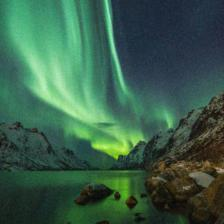
\includegraphics[width = 3.5cm]{imgs/no_fire.jpg} & 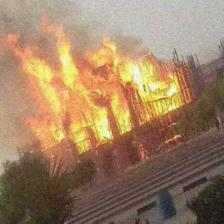
\includegraphics[width = 3.5cm]{imgs/fire.jpg}
        \\
        \texttt{label: 0} & \texttt{label: 1}
    \end{tabular}
    \caption{Example of images belonging to the dataset with the corresponding label}
\end{figure}

For this task, we used a dataset composed of $10,926$ images; we later applied some steps of data augmentation so that we could achieve better results by making the model generalize enough.
\nl
The dataset is separated in two folders (for the two classes), where each folder represents the label of each image:
\begin{itemize}
    \item folder \verb|0| contains the images that do not contain fire;
    \item folder \verb|1| contains the images that contain fire;
\end{itemize}

\subsection{Data augmentation}

Data augmentation is a common step which is usually made to enhance the number of items in a dataset by using items already belonging to said dataset. We applied the following operations to our dataset:
\begin{itemize}
    \item \textbf{Random rotation}: to each image, a random rotation of $x$ degrees could've been applied, where $x \in [0, 15]$. This ensures that the fire would be recognized even if it was not "parallel" with respect to the $y$ axis of the image;
    \item \textbf{Color jitter}: a random color jitter was also applied to all the images. The parameters passed to the jitter function are listed on Table \ref{color_jittering_vals}. By applying a color jitter, we make sure that the model would recognize a fire also when light conditions were not optimal in the photo (for instance if the image is either too dark or too bright);
    \item \textbf{Brightness noise}: for each image also some noise was added, and this was applied through a lambda function. For each image, some noise of equal size would be generated, and then through clamping the noise got applied to the image. This kind of noise allowed us to train the model to recognize a fire also in some harsh conditions, and helps avoiding overfitting.
\end{itemize}
\nl
After augmenting the whole dataset, the amount of samples went from $10,926$ to $21,852$, doubling the size of the dataset and allowing the models to train and reach more efficient results.

\begin{table}
    \caption{Parameters of the color jittering function}
    \label{color_jittering_vals}
    \centering
    \begin{tabular}{|l|c|}
        \hline
        \makecell{\textbf{Parameter}} & \textbf{Value}
        \\ \hline\hline
        \verb|brightness| & 0.2 \\ \hline
        \verb|contrast| & 0.2 \\ \hline
        \verb|saturation| & 0.2 \\ \hline
        \verb|hue| & 0.1 \\ \hline
    \end{tabular}
\end{table}

\section{Structure of the ensemble}

The ensemble is composed of three models, based on a ResNet 152, a ResNet 18 and a ResNet 50. The complete specifications of the three models can be found in Table \ref{ensemble_specs}. Some small modifications have been made to each model, in order to achieve different results. We here list all the modifications that have been made to each model, alongside an explanation of why they have been applied.
\nl
For the performance evaluation process, the predictions from the three models could be combined in many ways:
\begin{itemize}
    \item \textbf{Average}: in average mode, the outputs from the three models are averaged together, and this result represents the output of the ensemble. This is the method that we used;
    \item \textbf{Weighted average}: the outputs from the three models are averaged based on some given weights. This can be useful in case we consider the "opinion" of some models more meaningful than the others';
    \item \textbf{Vote}: the class considered to be the "most likely" by the majority of the outputs of the three models will be the class returned by the ensemble.
\end{itemize}

\subsection*{Model 1 \texorpdfstring{\textbullet}{•} ResNet 152}

In order to perform this classification, we started with a solid network, which originally was going to be the only network. After a throughout evaluation, we ultimately decided to create a model ensemble.
\nl
The ResNet 152 model also got some modifications on our end, such as the addition of two linear layers at the end of the network. The fore-last layer is connected to the output of the ResNet with a dropout of $0.5$, and uses the ReLU as an activation function; the last layer is connected to the previous layer with a dropout of $0.5$ and has two final neurons, one for each class (so one which stands for class \texttt{0}: \texttt{no fire} and one for class \texttt{1}: \texttt{fire}).
\nl
This model employs the focal loss function (implemented manually, in the Jupyter notebook present in the code repository) and the AdamW optimizer. Moreover, it was trained on the augmented dataset.
\nl
The reason why we decided to employ a ResNet 152 is that it's a stable, valid network: the ResNet model proved to be an important network, that could be easily adapted to our needs. This was a key point of our work: by using a pre-trained model and adding a few layers, we were able to construct a model which could fit very well our use case and that performs better than other architectures, by needing less training time;
%\item Lorenzo wanted to do it.

\subsection*{Models 2 \texorpdfstring{\&}{&} 3 \texorpdfstring{\textbullet}{•} ResNet 50 and ResNet 18}

The other two models for the ensemble are a ResNet 50 and a ResNet 18, without any additional layer. There are several reasons for this choice:
\begin{itemize}
    \item \textbf{Feasible}: using shallower models than ResNet 152 makes the training process faster;
    \item \textbf{Performance}: both models still provide a very good accuracy score on the validation set; % :P
    \item \textbf{Meaningful}: the structural difference between this two models and ResNet 152 is crucial to have meaningful changes in the feature space, which are reflected in the output of the models;
    \item \textbf{Dataset differences}: we didn't apply data augmentation for ResNet 50: the change of the used datasets for training does not affect negatively the accuracy score and improves the difference between the two models behavior, in order to have a reasonable ensemble. 
\end{itemize}

%\subsection*{Model 3 \texorpdfstring{\textbullet}{•} ResNet 18}

% model ensemble: 
% - resnet152
% - resnet18
% - resnet50

\begin{table*}[h!]
    \renewcommand{\arraystretch}{1.3}
    \caption{Structure of the ensemble}
    \label{ensemble_specs}
    \centering
    \begin{tabular}{|c|c|c|c|c|c|}
        \hline
        \textbf{Model} & \textbf{Layer} & \textbf{Dimension} & \textbf{Loss function} & \textbf{Optimizer} & \textbf{Data augmentation?} \\
        \hline
        \hline
        \multirow{5}{*}{ResNet 152} & \multicolumn{2}{c|}{Backbone of the ResNet 152} & \multirow{5}{*}{Focal Loss} & \multirow{5}{*}{AdamW} & \multirow{5}{*}{$\checkmark$}
        \\ \cline{2-3} 
        & Dropout & $0.5$ & & &
        \\
        & Linear (ReLU) & $(1024 \times 512)$ & & &
        \\
        & Dropout & $0.5$ & & &
        \\
        & Linear & $(512 \times 2)$ & & &
        \\
        \hline\hline
        \multirow{1}{*}{ResNet 50} & \multicolumn{2}{c|}{Backbone of the ResNet 50} & \multirow{1}{*}{Cross Entropy Loss} & \multirow{1}{*}{SGD} & \multirow{1}{*}{$\times$}
        \\
        \hline \hline
        \multirow{1}{*}{ResNet 18} & \multicolumn{2}{c|}{Backbone of the ResNet 18} & \multirow{1}{*}{Focal Loss} & \multirow{1}{*}{SGD} & \multirow{1}{*}{$\checkmark$}
        \\
        \hline
    \end{tabular}
    \nl
    \begin{tabular}{c c}
        $\checkmark$: Yes & $\times$: No 
    \end{tabular}
\end{table*}

\pagebreak

\section{Performance evaluation}

The performance for the ensemble and the singular models that we described in this paper can be found in Table \ref{ensemble_performance}.
\nl
Unfortunately, the difference in accuracy between the singular models and the ensemble is not as large as desired, but it's still an improvement over the single-model approach.

\begin{table}[h!]
    \caption{Performance of the ensemble and the three models}
    \label{ensemble_performance}
    \centering
    \begin{tabular}{|c|c|}
        \hline
        \textbf{Model} & \textbf{Accuracy} \\
        \hline\hline
        ResNet 152 & $98.46\%$ \\
        \hline
        ResNet 18 & $98.49\%$ \\
        \hline
        ResNet 50 & $98.75\%$ \\
        \hline
        Average of the ensemble & $98.81\%$ \\
        \hline
    \end{tabular}
    \nl
    {\scriptsize The items have been listed in ascending order of accuracy}
\end{table}

\printbibliography

\end{document}